\documentclass[a4paper,10pt]{article}
\usepackage[T1]{fontenc}
\usepackage[utf8]{inputenc}
\usepackage[slovene]{babel}
\usepackage[margin=1.3cm]{geometry}
\usepackage{amsmath,amssymb}
\usepackage{graphicx}
\usepackage{enumitem}
\usepackage{tikz}
\usepackage{xcolor}
\usepackage{titlesec}
\usepackage{hyperref}
\usepackage[most]{tcolorbox}
\usetikzlibrary{arrows.meta}

\definecolor{barvaNaslovov}{HTML}{245B78}
\definecolor{barvaPomembno}{HTML}{B3261E}
\definecolor{barvaPrimerov}{HTML}{626B73}
\definecolor{barvaNaslovaPrimera}{HTML}{454B50}
\definecolor{barvaDrugiVektor}{HTML}{39835A}
\definecolor{barvaModra}{HTML}{EAF3FB}
\definecolor{barvaZelena}{HTML}{EAF8EE}
\definecolor{barvaRdeca}{HTML}{FDECEC}
\definecolor{barvaRumena}{HTML}{FFF7DE}

\titleformat{\section}{\large\bfseries\color{barvaNaslovov}}{\thesection}{0.7em}{}
\titleformat{\subsection}{\normalsize\bfseries\color{barvaNaslovov}}{\thesubsection}{0.7em}{}
\titlespacing*{\section}{0pt}{0.55em}{0.25em}
\titlespacing*{\subsection}{0pt}{0.35em}{0.20em}
\setlist[itemize]{leftmargin=1.1em,itemsep=2pt,topsep=2pt,parsep=0pt,partopsep=0pt}
\setlength{\parskip}{1.5pt}
\setlength{\parindent}{0pt}
\setlength{\abovedisplayskip}{3pt}
\setlength{\belowdisplayskip}{3pt}
\setlength{\abovedisplayshortskip}{2pt}
\setlength{\belowdisplayshortskip}{2pt}
\hypersetup{colorlinks=true,linkcolor=barvaNaslovov,urlcolor=barvaNaslovov}

\newcommand{\vect}[1]{\vec{#1}}
\newcommand{\abs}[1]{|#1|}
\newcommand{\pomembno}[1]{\textcolor{barvaPomembno}{#1}}
\newenvironment{primer}{\par\begingroup\color{barvaPrimerov}}{\par\endgroup}

\newtcolorbox{bluecard}[2][]{enhanced, breakable,
    colback=barvaModra,
    colframe=barvaNaslovov,
    boxrule=0.6pt,
    arc=2mm,
    left=6pt,right=6pt,top=5pt,bottom=5pt,
    title={\bfseries #2},
    coltitle=white,
    colbacktitle=barvaNaslovov,
    attach boxed title to top left={xshift=5mm,yshift=-2mm},
    boxed title style={boxrule=0pt, arc=2mm},
    #1
}
\newtcolorbox{greencard}[2][]{enhanced, breakable,
    colback=barvaZelena,
    colframe=barvaDrugiVektor,
    boxrule=0.6pt,
    arc=2mm,
    left=6pt,right=6pt,top=5pt,bottom=5pt,
    title={\bfseries #2},
    coltitle=white,
    colbacktitle=barvaDrugiVektor,
    attach boxed title to top left={xshift=5mm,yshift=-2mm},
    boxed title style={boxrule=0pt, arc=2mm},
    #1
}
\newtcolorbox{redcard}[2][]{enhanced, breakable,
    colback=barvaRdeca,
    colframe=barvaPomembno,
    boxrule=0.6pt,
    arc=2mm,
    left=6pt,right=6pt,top=5pt,bottom=5pt,
    title={\bfseries #2},
    coltitle=white,
    colbacktitle=barvaPomembno,
    attach boxed title to top left={xshift=5mm,yshift=-2mm},
    boxed title style={boxrule=0pt, arc=2mm},
    #1
}
\newtcolorbox{yellowcard}[2][]{enhanced, breakable,
    colback=barvaRumena,
    colframe=barvaNaslovaPrimera,
    boxrule=0.6pt,
    arc=2mm,
    left=6pt,right=6pt,top=5pt,bottom=5pt,
    title={\bfseries #2},
    coltitle=white,
    colbacktitle=barvaNaslovaPrimera,
    attach boxed title to top left={xshift=5mm,yshift=-2mm},
    boxed title style={boxrule=0pt, arc=2mm},
    #1
}
\newtcolorbox{graycard}[2][]{enhanced, breakable,
    colback=gray!15,
    colframe=gray!60,
    boxrule=0.6pt,
    arc=2mm,
    left=6pt,right=6pt,top=5pt,bottom=5pt,
    title={\bfseries #2},
    coltitle=white,
    colbacktitle=gray!70,
    attach boxed title to top left={xshift=5mm,yshift=-2mm},
    boxed title style={boxrule=0pt, arc=2mm},
    #1
}

\begin{document}

\title{\vspace{-1em}\Large\bfseries Pregled snovi: Vektorji}
\author{}
\date{}
\maketitle\vspace{-1.8em}

\section{Osnove o vektorjih}
\begin{bluecard}{Definicija}
\vspace{0pt}
\begin{minipage}[t]{0.58\textwidth}
Vektor je določen s smerjo, usmerjenostjo in dolžino.
\medskip

\textbf{Oznaka:} Vektor označimo z $\vect{AB}$ ali z $\vect{a}$.
\medskip

\textbf{Dolžina:} $\abs{\vect{a}}$.
\medskip

\textbf{Enaka vektorja} so vzporedna, enako dolga in enako usmerjena.
\medskip

\textbf{Nasprotni vektor} $-\vect{a}$ je enako dolg, a usmerjen v nasprotno smer.
\medskip

\textbf{Ničelni vektor} $\vect{0}$ ima dolžino $0$.
\end{minipage}\hfill
\begin{minipage}[t]{0.38\textwidth}
\vspace{0pt}
\centering
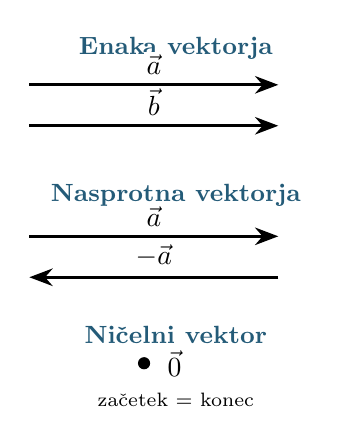
\begin{tikzpicture}[x=0.62cm,y=0.52cm,>=Stealth]
    \node[font=\small\bfseries, text=barvaNaslovov] at (3.4,7.8) {Enaka vektorja};
    \draw[->,line width=1.2pt] (0.4,6.9) -- (5.5,6.9) node[midway,above=2pt,fill=white,inner sep=1pt] {$\vect{a}$};
    \draw[->,line width=1.2pt] (0.4,5.9) -- (5.5,5.9) node[midway,above=2pt,fill=white,inner sep=1pt] {$\vect{b}$};
    \node[font=\small\bfseries, text=barvaNaslovov] at (3.4,4.2) {Nasprotna vektorja};
    \draw[->,line width=1.2pt] (0.4,3.2) -- (5.5,3.2) node[midway,above=2pt,fill=white,inner sep=1pt] {$\vect{a}$};
    \draw[->,line width=1.2pt] (5.5,2.2) -- (0.4,2.2) node[midway,above=2pt,fill=white,inner sep=1pt] {$-\vect{a}$};
    \node[font=\small\bfseries, text=barvaNaslovov] at (3.4,0.8) {Ničelni vektor};
    \fill (2.75,0.1) circle (2.2pt);
    \node[right=5pt] at (2.75,0.1) {$\vect{0}$};
    \node[font=\scriptsize] at (3.4,-0.8) {začetek = konec};
\end{tikzpicture}
\end{minipage}
\end{bluecard}

\section{Seštevanje in odštevanje vektorjev}
\begin{greencard}{Grafično seštevanje}
Vektorja seštejemo po pravilu trikotnika ali po pravilu paralelograma.

\begin{minipage}[t]{0.48\textwidth}
\centering
\textbf{Trikotniško pravilo}\par\smallskip
Začetek $\vect{b}$ postavimo v konec $\vect{a}$.
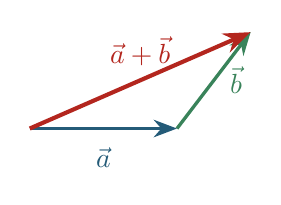
\begin{tikzpicture}[x=0.85cm,y=0.72cm,>=Stealth]
    \coordinate (O) at (0,0);\coordinate (A) at (2.2,0);\coordinate (C) at (3.3,1.7);
    \draw[->,line width=1.2pt,barvaNaslovov] (O) -- (A) node[midway,below=3pt] {$\vect{a}$};
    \draw[->,line width=1.2pt,barvaDrugiVektor] (A) -- (C) node[midway,right=2pt] {$\vect{b}$};
    \draw[->,line width=1.5pt,barvaPomembno] (O) -- (C) node[midway,above=1pt] {$\vect{a}+\vect{b}$};
\end{tikzpicture}
\end{minipage}\hfill
\begin{minipage}[t]{0.48\textwidth}
\centering
\textbf{Paralelogramsko pravilo}\par\smallskip
Vektorja začneta v isti točki.
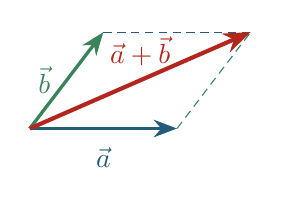
\begin{tikzpicture}[x=0.85cm,y=0.72cm,>=Stealth]
    \coordinate (O) at (0,0);\coordinate (A) at (2.2,0);\coordinate (B) at (1.1,1.7);\coordinate (C) at (3.3,1.7);
    \draw[->,line width=1.2pt,barvaNaslovov] (O) -- (A) node[midway,below=3pt] {$\vect{a}$};
    \draw[->,line width=1.2pt,barvaDrugiVektor] (O) -- (B) node[midway,left=2pt] {$\vect{b}$};
    \draw[densely dashed,barvaNaslovov] (B) -- (C);\draw[densely dashed,barvaDrugiVektor] (A) -- (C);
    \draw[->,line width=1.5pt,barvaPomembno] (O) -- (C) node[midway,above=1pt] {$\vect{a}+\vect{b}$};
\end{tikzpicture}
\end{minipage}
\end{greencard}

\begin{minipage}[t]{0.48\textwidth}
\begin{yellowcard}{Lastnosti}
\begin{itemize}
    \item komutativnost: $\vect{a}+\vect{b}=\vect{b}+\vect{a}$,
    \item asociativnost: $(\vect{a}+\vect{b})+\vect{c}=\vect{a}+(\vect{b}+\vect{c})$,
    \item nevtralni element: $\vect{a}+\vect{0}=\vect{a}$,
    \item nasprotni element: $\vect{a}+(-\vect{a})=\vect{0}$.
\end{itemize}
\end{yellowcard}
\end{minipage}\hfill
\begin{minipage}[t]{0.48\textwidth}
\begin{redcard}{Odštevanje}
\textbf{Odštevanje:} $\pomembno{\vect{a}-\vect{b}=\vect{a}+(-\vect{b})}$.
\vspace{2mm}
\centering
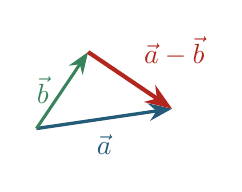
\begin{tikzpicture}[x=0.82cm,y=0.72cm,>=Stealth]
    \coordinate (O) at (0,0);
    \coordinate (A) at (2.1,0.35);
    \coordinate (B) at (0.8,1.35);
    \draw[->,line width=1.2pt,barvaNaslovov] (O) -- (A)
        node[midway,below=2pt] {$\vect{a}$};
    \draw[->,line width=1.1pt,barvaDrugiVektor] (O) -- (B)
        node[midway,left=1pt] {$\vect{b}$};
    \draw[->,line width=1.5pt,barvaPomembno] (B) -- (A)
        node[midway,above right=1pt] {$\vect{a}-\vect{b}$};
\end{tikzpicture}
\end{redcard}
\end{minipage}

\section{Množenje vektorja s skalarjem}
\begin{redcard}{Skalar in smer}
\vspace{0pt}
\begin{minipage}[t]{0.54\textwidth}
Skalar je realno število. Vektor $\vect{a}$ pomnožen s $k$ zapišemo kot $\pomembno{k\vect{a}}$.
\begin{itemize}
    \item $\pomembno{\abs{k\vect{a}}=|k|\,\abs{\vect{a}}}$,
    \item $k>0$: ista usmerjenost,
    \item $k<0$: nasprotna usmerjenost,
    \item $k=0$: ničelni vektor.
\end{itemize}
\end{minipage}\hfill
\begin{minipage}[t]{0.4\textwidth}
\vspace{0pt}
\centering
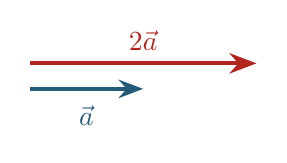
\begin{tikzpicture}[x=0.72cm,y=0.72cm,>=Stealth]
    \draw[->,line width=1.3pt,barvaNaslovov] (0,0) -- (2,0) node[midway,below=2pt] {$\vect{a}$};
    \draw[->,line width=1.5pt,barvaPomembno] (0,0.45) -- (4,0.45) node[midway,above=3pt,fill=white,inner sep=1pt] {$2\vect{a}$};
\end{tikzpicture}
\end{minipage}
\end{redcard}

\section{Komponente vektorja}
\begin{bluecard}{Koordinatni zapis}
\vspace{0pt}
\begin{minipage}[t]{0.56\textwidth}
Vektor lahko zapišemo s komponentami v koordinatnem sistemu:
\[
\pomembno{\vect{a}=(a_1,a_2)=a_1\vect{i}+a_2\vect{j}.}
\]
\begin{itemize}
    \item seštevanje: $\pomembno{\vect{a}+\vect{b}=(a_1+b_1,a_2+b_2)}$,
    \item odštevanje: $\pomembno{\vect{a}-\vect{b}=(a_1-b_1,a_2-b_2)}$,
    \item množenje s skalarjem: $\pomembno{k\vect{a}=(ka_1,ka_2)}$.
\end{itemize}
\end{minipage}\hfill
\begin{minipage}[t]{0.38\textwidth}
\vspace{0pt}
\centering
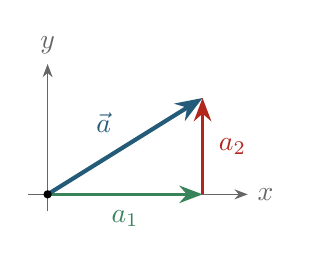
\begin{tikzpicture}[x=0.82cm,y=0.72cm,>=Stealth]
    \coordinate (O) at (0,0);\coordinate (X) at (2.4,0);\coordinate (A) at (2.4,1.7);
    \draw[->,gray!80!black] (-0.3,0) -- (3.1,0) node[right] {$x$};
    \draw[->,gray!80!black] (0,-0.3) -- (0,2.3) node[above] {$y$};
    \draw[densely dashed,gray] (A) -- (X);
    \draw[->,line width=1.2pt,barvaDrugiVektor] (O) -- (X) node[midway,below=2pt] {$a_1$};
    \draw[->,line width=1.2pt,barvaPomembno] (X) -- (A) node[midway,right=2pt] {$a_2$};
    \draw[->,line width=1.5pt,barvaNaslovov] (O) -- (A) node[midway,above left=1pt] {$\vect{a}$};
    \fill (O) circle (1.5pt);
\end{tikzpicture}
\end{minipage}
\end{bluecard}

\begin{graycard}{Primer}
Če je $\vect{a}=(2,3)$ in $\vect{b}=(1,1)$, potem
\[
\vect{a}+\vect{b}=(3,4),
\quad
\vect{a}-\vect{b}=(1,2),
\quad
2\vect{a}=(4,6).
\]
\end{graycard}

\begin{greencard}{Dolžina vektorja}
Dolžina vektorja $\vect{AB}$ je razdalja med točkama $A$ in $B$:
\[
\pomembno{\abs{\vect{AB}}=d(A,B)=\sqrt{(b_1-a_1)^2+(b_2-a_2)^2}}.
\]
\textbf{Primer:} $A(1,2)$, $B(4,5)$, zato
\[
\abs{\vect{AB}}=\sqrt{(4-1)^2+(5-2)^2}=\sqrt{9+9}=3\sqrt{2}.
\]
\end{greencard}

\begin{minipage}[t]{0.48\textwidth}
\begin{redcard}{Enotski vektor}
Enotski vektor v smeri $\vect{a}$ ima dolžino $1$:
\[
\pomembno{\vect{a}_e=\frac{1}{\abs{\vect{a}}}\vect{a},\qquad \abs{\vect{a}_e}=1.}
\]
\end{redcard}
\end{minipage}\hfill
\begin{minipage}[t]{0.48\textwidth}
\begin{graycard}{Primer}
Za $\vect{a}=(3,4)$ je $\abs{\vect{a}}=5$, torej
\[
\vect{a}_e=\left(\frac35,\frac45\right).
\]
\end{graycard}
\end{minipage}

\section{Baza in linearne kombinacije}
\begin{greencard}{Baza ravnine in prostora}
Linearna kombinacija vektorjev $\vect{a}$ in $\vect{b}$ je izraz oblike
\[
\pomembno{\alpha\vect{a}+\beta\vect{b},\quad \alpha,\beta\in\mathbb{R}.}
\]
Dva neodvisna vektorja tvorita bazo ravnine, trije pa bazo prostora.
\[
\pomembno{\vect{v}=x\vect{a}+y\vect{b}}, \qquad
\pomembno{\vect{v}=x\vect{a}+y\vect{b}+z\vect{c}}.
\]
\end{greencard}

\section{Odvisni in neodvisni vektorji}
\begin{bluecard}{Definicija}
Vektorja $\vect{a}$ in $\vect{b}$ sta linearno neodvisna, če iz
\[
\alpha\vect{a}+\beta\vect{b}=\vect{0}
\]
sledi $\alpha=\beta=0$.
\begin{itemize}
    \item če sta vzporedna, sta linearno odvisna,
    \item v ravnini potrebujemo dva neodvisna vektorja za bazo.
\end{itemize}
\end{bluecard}

\begin{graycard}{Primer}
Vektorja $\vect{a}=(2,3)$ in $\vect{b}=(4,1)$ sta neodvisna, saj edina rešitev sistema
\[
\begin{cases}
2\alpha+4\beta=0,\cr
3\alpha+\beta=0
\end{cases}
\]
je $\alpha=\beta=0$.
\end{graycard}

\section{Skalarni produkt}
\begin{redcard}{Definicija in lastnosti}
Skalarni produkt dveh vektorjev je število:
\[
\pomembno{\vect{a}\cdot\vect{b}=\abs{\vect{a}}\,\abs{\vect{b}}\cos\varphi.}
\]
\begin{itemize}
    \item komutativnost: $\vect{a}\cdot\vect{b}=\vect{b}\cdot\vect{a}$,
    \item distributivnost: $\vect{a}\cdot(\vect{b}+\vect{c})=\vect{a}\cdot\vect{b}+\vect{a}\cdot\vect{c}$,
    \item homogenost: $(k\vect{a})\cdot\vect{b}=k(\vect{a}\cdot\vect{b})$.
\end{itemize}
\end{redcard}

\begin{greencard}{Pomen}
\begin{itemize}
    \item $\varphi=90^\circ \Rightarrow \vect{a}\cdot\vect{b}=0$ (pravokotna),
    \item $\varphi=0^\circ \Rightarrow \vect{a}\cdot\vect{b}=\abs{\vect{a}}\abs{\vect{b}}$,
    \item $\varphi=180^\circ \Rightarrow \vect{a}\cdot\vect{b}=-\abs{\vect{a}}\abs{\vect{b}}$.
\end{itemize}
\end{greencard}

\begin{graycard}{Primer}
Če je $\vect{a}=(a_1,a_2,a_3)$ in $\vect{b}=(b_1,b_2,b_3)$, potem
\[
\pomembno{\vect{a}\cdot\vect{b}=a_1b_1+a_2b_2+a_3b_3.}
\]
Na primer:
\[
(3,4)\cdot(1,2)=3\cdot1+4\cdot2=11.
\]
\end{graycard}

\section{Povzetek}
\begin{tcolorbox}[enhanced, colback=white, colframe=barvaNaslovov, boxrule=0.8pt, arc=2mm, left=8pt,right=8pt,top=6pt,bottom=6pt]
\begin{itemize}
    \item vektor ima smer, usmerjenost in dolžino,
    \item seštevanje in odštevanje uporabljata pravila trikotnika/paralelograma,
    \item množenje s skalarjem spremeni dolžino in lahko obrne smer,
    \item linearno neodvisni vektorji tvorijo bazo,
    \item skalarni produkt je število, povezano z dolžinami in kotom,
    \item s komponentami je računanje z vektorji najpreprostejše.
\end{itemize}
\end{tcolorbox}

\end{document}
